\section{\iflanguage{english}{Implementation}{Implementierung}}

\subsection{\iflanguage{english}{Designing the Kernel's interface}{Entwurf der 
Schnittstelle des Kernels}}

Many implementations of linear algebra routines in OpenCL strive for maximal 
performance and therefore restrict their operands to special dimensions, sizes 
and layout. If these implementations are integrated into software packages like 
MATLAB, copying and other preprocessing respectively is required to meet the 
implementations' requirements. This in turn hinders performance. Therefore the 
kernel presented here has a more flexible interface eventhough this may provoke 
a slower execution.

In the C++ standard library when abstracting away the actual layout and size of 
a data structure iterators are used. As OpenCL is a C derivative rather than a 
C++ derivative, iterators can not be used directly if they are more complex 
than simple pointers. Instead several parameters are handed over to the kernel 
that define the iterator. In \cite{Volkov2008} the kernel launch overhead has 
been measured for CUDA and in \cite{Dongarra2013} for OpenCL but not with 
respect to the number of parameters passed to the kernel. In 
\cref{fig:kernelLaunchOverhead} the kernel launch overhead for the three major 
hardware platforms mentioned in \cref{sec:hardware} is presented varying the 
number of parameters from one to 32 which should cover the most common kernel 
invocations. The test was done executing an empty kernel several thousand times 
and then averaging the execution time. As one can see there is a linear 
correspondence between the number of kernel arguments and the launch overhead. 
Thus one should use parameters sparingly. To reduce the number of kernel 
arguments 
one could place them in continuous global memory and just pass the address of 
the first. But that requires extra loading from global memory. Therefore it is 
not used here.

\begin{figure}[htbp]
 \centering
 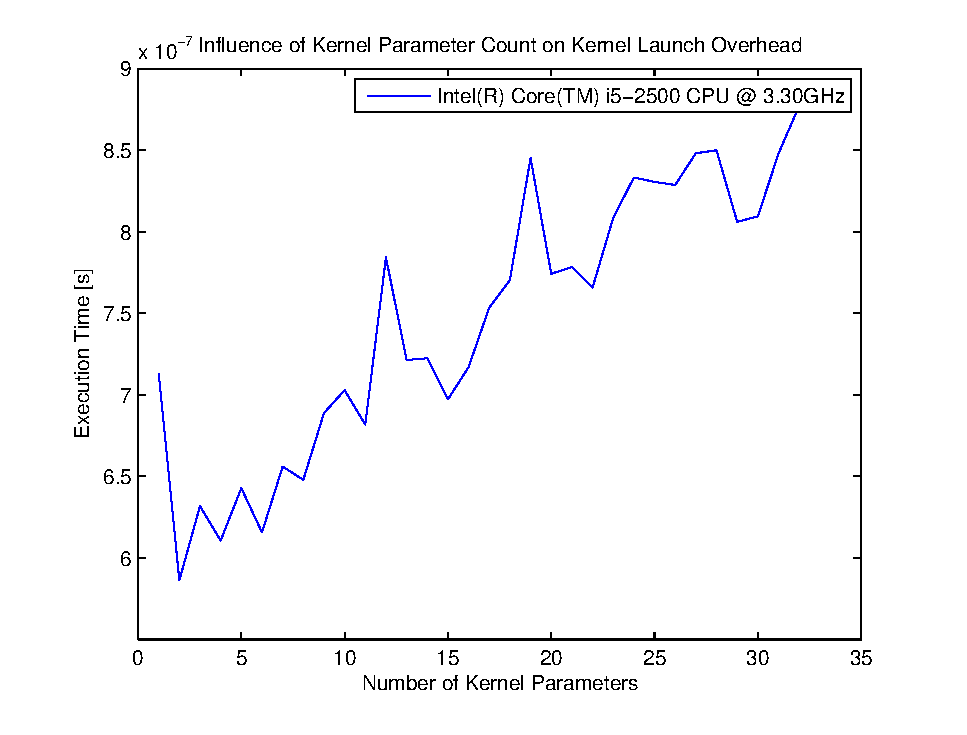
\includegraphics[width=\textwidth]{kernelLaunchOverhead}
 \caption{Impact of the Number of Parameters on Kernel Launch Overhead}
 \label{fig:kernelLaunchOverhead}
\end{figure}

The kernel presented in \cref{lst:kernelHeader} has parameters to access all 
three matrices or submatrices and hides the layout\footnote{This design allows 
column- and row-major layouts only.} of them by additional parameters.

Both operands are qualified with the \texttt{const} keyword to indicate that 
they are read-only. This helps in avoiding unintentional writes and in
optimization. All three pointers are restricted. That enables further 
optimizations on some devices \footnote{E.g.\ AMD Nothern Islands \acp{GPU} 
enable caching only for restricted pointers to read-only 
memory\cite[Section 7.4]{AMD2013}}. The \texttt{restrict} keyword requires that 
\texttt{lhs}, \texttt{rhs} and \texttt{res} do not alias. \texttt{res} must 
point to a distinct memory location because if it was one of the operands 
updating it must be delayed until all reads are done. That would require 
synchronization of all work items which in general is not possible. 
\texttt{lhs} and \texttt{rhs} may alias allowing computations of the form $C = 
A \cdot A$ because they are not updated at all due to the \texttt{const} 
qualifier.

Even though OpenCL does not support templates directly, C++-style 
templatization is used here to indicate that the kernel can be implemented for 
various types.

The offsets mark the beginning of the (sub-) matrices and the stride parameters 
hide column- or row-major data layout of the matrices.

\texttt{innerDim} is the size of the common dimension of the left- and 
right-hand side operand.
\begin{lstlisting}[caption={Interface of the OpenCL kernel for matrix-matrix 
multiplication},label={lst:kernelHeader},language=OpenCL]
template<class T>
kernel void gemm(
  global T const* restrict lhs, // left-hand side (sub-)matrix
  global T const* restrict rhs, // right-hand side (sub-)matrix
  global T* const restrict res, // result (sub-) matrix
  uint const      innerDim,   // inner dimension of lhs and rhs
  uint const      lhsOffset,  // offset into lhs where the 
                              // (sub-) matrix begins
  uint const      rhsOffset,  // same for rhs
  uint const      resOffset,  // same for res
  uint const      lhsStrideX, // distance between consecutive lhs
                              // values in horizontal direction
  uint const      rhsStrideX, // same for rhs
  uint const      resStrideX, // same for res
  uint const      lhsStrideY, // distance between consecutive lhs
                              // values in vertical direction
  uint const      rhsStrideY, // same for rhs
  uint const      resStrideY  // same for lhs
);\end{lstlisting}

Besides global memory OpenCL permits storing data in the texture cache, if the 
device supports that. To make use of the texture cache a second kernel 
interface is presented in \cref{lst:kernelHeaderImgMem}. It supports matrices 
that are stored as textures. On some devices like AMD's Nothern Island 
\acp{GPU} the texture cache has a higher bandwidth than the global memory 
\cite[Section 7.4]{AMD2013}. 

Textures in OpenCL are two- or three-dimensional arrays that store four values 
per texel\footnote{A value for red, green, blue and alpha intensity}. Their 
exact memory layout is not specified such that each implementation can apply 
its own customizations or optimizations respectively. On the other hand images 
stored in host memory are required to be laid out row by row and one to four 
continuous values form one texel. When the image is moved to the texture memory 
missing values are added as specified by the programmer. E.g. if the programmer 
specified that the image in host memory is of the format \texttt{CL\_LUMINANCE} 
then one value in host memory is copied and duplicated into image memory such 
that the resulting texel has the value $\begin{pmatrix}L,L,L,1.0\end{pmatrix}$. 
If the image has been given the channel order \texttt{CL\_RGBA} then four 
values in host memory are copied into one texel in image memory of the form 
$\begin{pmatrix}R,G,B,A\end{pmatrix}$.

As stated above, the layout of images in image memory is not specified. Images 
can not be accessed like arrays inside a kernel but by two- or 
three-dimensional coordinates. Thus the offset parameters slightly differ from 
the kernel in \cref{lst:kernelHeader}. Logically the strides in both direction 
are one. If the matrix was not in row- but in column-major format before 
copying it into image memory this is indicated by the \texttt{transpose} 
parameter.

% TODO Encoding of textures as matrices.

\begin{lstlisting}[caption={Interface of the OpenCL kernel for matrix-matrix 
multiplication using image 
memory},label={lst:kernelHeaderImgMem},language=OpenCL]
kernel void gemm(
  read_only  image2d_t lhs,
  read_only  image2d_t rhs,
  write_only image2d_t res,
  int const            innerDim,
  int const            lhsOffsetX,
  int const            rhsOffsetX,
  int const            resOffsetX,
  int const            lhsOffsetY,
  int const            rhsOffsetY,
  int const            resOffsetY,
  int const            lhsTranspose, // Was the matrix in host
                                     // memory stored in column-
                                     // or row-major format?
  int const            rhsTranspose,
  int const            resTranspose
);\end{lstlisting}


% TODO Test how more parameters influence the time it takes to invoke a kernel.